\documentclass[11pt]{tingpset}

\Name                   {Michaels Tingley and Traver}
\Email                  {\{michaeltingley, mtraver\}@college.harvard.edu}
\Organization           {Harvard University}
\Class                  {Computer Science 175}
\ClassShort             {CS175}
\ProblemSetNumber       {1.5}
\DueDate                {30 September 2013, 11:59pm}
\CollaborationStatement {Michaels Tingley and Traver completed this problem set in tandem.}

\begin{document}
  \makeheader

  %%%%%%%%%%%%%%%%%%%%%%%%%%%% 4.1 %%%%%%%%%%%%%%%%%%%%%%%%%%%%
  \problemn{4.1}
  First we consider the ``local'' interpretation, rotating and then translating with respect to the intermediate frame for each transformation:
  \begin{center}
    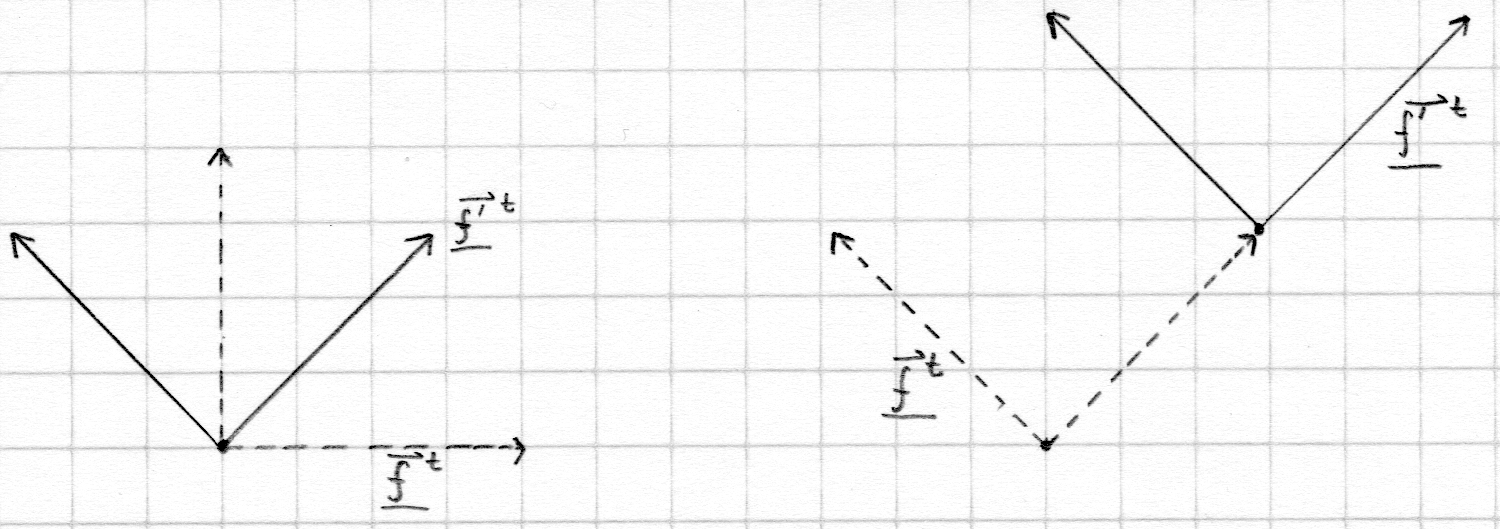
\includegraphics[width=11cm]{CS175_asst1_5_1a}
  \end{center}

  Next we consider the ``global'' interpretation, translating and then rotating with respect to the original frame for all transformations:
  \begin{center}
    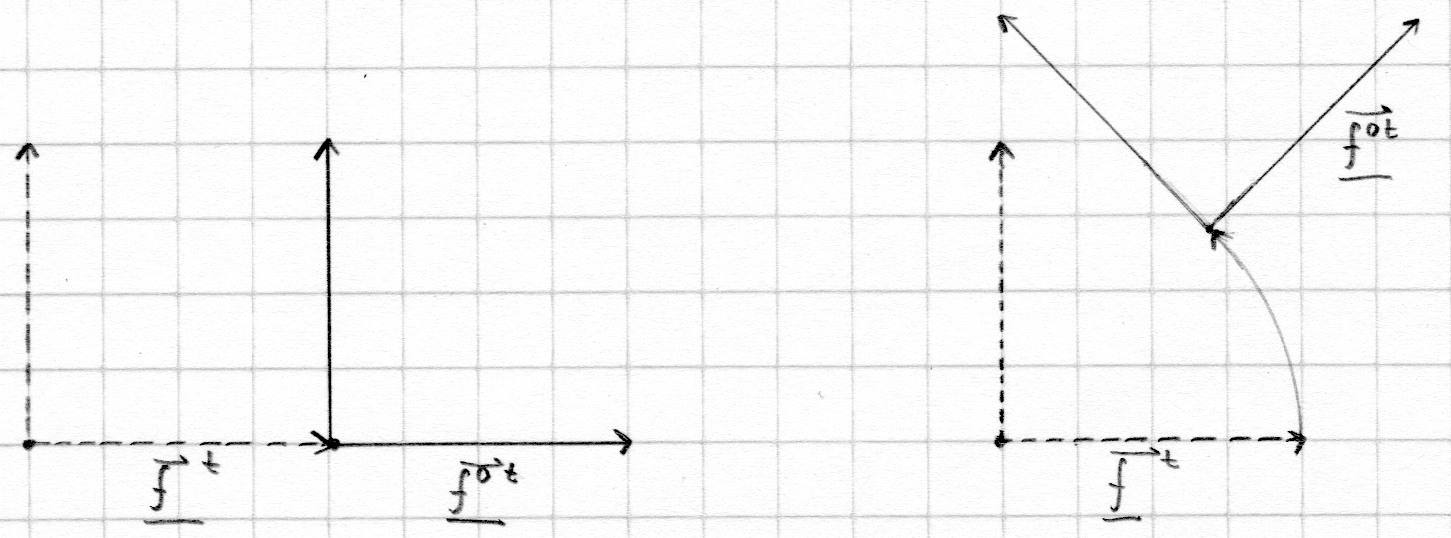
\includegraphics[width=11cm]{CS175_asst1_5_1b}
  \end{center}

  As we expect, each interpretation yields the same final frame.

  %%%%%%%%%%%%%%%%%%%%%%%%%%%% 4.2 %%%%%%%%%%%%%%%%%%%%%%%%%%%%
  \problemn{4.2}
  The frame's origin moves 2 units. This can be visualized both locally and globally:
  \begin{description}
    \item[local:] The frame is first uniformly scaled by a factor of two, and then is translated by one unit in the enlarged frame's units. This results in the origin moving 2 units, in the original frame's units, along the $x$ axis.
    \item[global:] The frame is first translated 1 unit, and then scaled with respect to the original frame by a factor of 2. This results in the frame being ``pushed'' 1 unit along the $x$ axis as it is scaled, so again the origin moves a total of 2 units.
  \end{description}

  %%%%%%%%%%%%%%%%%%%%%%%%%%%% 4.3 %%%%%%%%%%%%%%%%%%%%%%%%%%%%
  \problemn{4.3}
    \renewcommand{\a}{\vec{\boldsymbol{a}}^t}
    \newcommand{\ap}{\vec{\boldsymbol{a}}'^t}
    \newcommand{\ao}{\vec{\boldsymbol{a}}^{\circ t}}
    \renewcommand{\b}{\vec{\boldsymbol{b}}^t}
    Note that in both of these scenarios, we have to rotate by $\theta$. So we have no choice but to set
    \[
      R=
        \begin{pmatrix}
          \cos{\theta} & -\sin{\theta} & 0 \\
          \sin{\theta} & \cos{\theta} & 0 \\
          0 & 0 & 1
       \end{pmatrix}.
    \]
    \textit{Realize that this will be true in all of the analyses below; the assignment of $R$ will not be repeated in the following discussions.}

    Now, we'll discuss $T$ in the equation $\b=\a TR$ in two ways. First, the local way gives the following interpretation:

    \ind{%
      Consider $\ap=\a T$. This means that ``$\ap$ is transformed by $T$ with respect to $\a$.'' Thus, $\ap$ is translated according to $T$ from its original position. We now consider $\b=\ap R$, which means ``$\b$ is transformed by $R$ with respect to $\ap$.'' We understand this description as: we are rotating (``applying $R$'') to our frame last, after having translated the frame that we are rotating around. So, since we have translated to get our intermediate frame, we realize that the translation is done in the direction of the original frame, and so we conclude that
      \[
        T=
          \begin{pmatrix}
            1 & 0 & d_1 \\
            0 & 1 & d_2 \\
            0 & 0 & 1
          \end{pmatrix}.
      \]
    }

    \noindent We can also consider the global interpretation:

    \ind{%
      Consider $\ao=\a R$. This means that ``$\ao$ is transformed by $R$ with respect to $\a$.'' Thus, $\ao$ is rotated according to $R$ about its original reference frame. We now consider $\b=\a T R$, which means ``$\ao$ is transformed by $T$ with respect to $\a$ --- its original reference frame.'' We understand this description as: we are rotating (``applying $R$'') to our frame first, and then translating (``applying $T$'') in terms of the original frame of reference. Since we are translating in the direction of the original frame, we conclude that
      \[
        T=
          \begin{pmatrix}
            1 & 0 & d_1 \\
            0 & 1 & d_2 \\
            0 & 0 & 1
          \end{pmatrix}.
      \]
    }

    \hrule

    Now, we'll discuss $T$ in the equation $\b=\a RT$ in two ways. First, the local way gives the following interpretation:

    \ind{
      Consider $\ap=\a R$. This means that ``$\ap$ is transformed by $R$ with respect to $\a$.'' Thus, $\ap$ is rotated according to $R$ from its original position. We now consider $\b=\ap T$, which means ``$\b$ is transformed by $T$ with respect to $\ap$.'' We understand this description as: we are translating (``applying $T$'') to our frame last, after having rotated the frame around its original reference frame. So, since we have rotated to get our intermediate frame, our translation has to be done with respect to this rotated reference frame, and we conclude that
      \[
        T=
          \begin{pmatrix}
            1 & 0 & d_3 \\
            0 & 1 & d_4 \\
            0 & 0 & 1
          \end{pmatrix}.
      \]
    }

    We can also consider the global interpretation:

    \ind{
      Consider $\ao=\a T$. This means that ``$\ao$ is transformed by $T$ with respect to $\a$.'' Thus, $\ao$ is translated according to $T$ from its original reference frame. We now consider $\b=\a R T$, which means ``$\ao$ is transformed by $R$ with respect to $\a$ --- its original reference frame.'' We understand this description as: we are translating (``applying $T$'') to our frame first, and then rotating (``applying $R$'') in terms of the original frame of reference. So we translate and then rotate. If we want to end up with the frame $\b$ given in the diagram, this means that we translate over $d_3$ and up $d_4$. Then, if we rotate around the \emph{original reference frame} by $\theta$, that will land us where $\b$ is given in the digram. So we conclude that
      \[
        T=
          \begin{pmatrix}
            1 & 0 & d_3 \\
            0 & 1 & d_4 \\
            0 & 0 & 1
          \end{pmatrix}.
      \]
    }

  %%%%%%%%%%%%%%%%%%%%%%%%%%%% 4.4 %%%%%%%%%%%%%%%%%%%%%%%%%%%%
  \problemn{4.4}
    \renewcommand{\a}{\vec{\boldsymbol{a}}^t}
    \renewcommand{\b}{\vec{\boldsymbol{b}}^t}
    \renewcommand{\c}{\vec{\boldsymbol{c}}^t}
    First, let's look at what we want to do here. We want to rotate $\a$ by $\theta$ around (``with respect to'') $\b$. Why is this? First, realize that the origin of $\a$ and $\c$ are both $d$ away from $b$'s origin. This means that they could `swing' along a rope of length $d$ tethered at $\b$'s origin and run into each other. This, however, doesn't guarantee that their orientations are the same. For this, we first need to realize that, from the assumptions that we are making in this class, $\a, \b,$ and $\c$ are orthogonal frames --- that is, their comprising vectors are orthogonal to each other. This is important, because it means that the angles between the two components of the frame form a right angle. Since the complement of the angle of measure $\phi$ must be the same in both $\a$ and $\c$ (since reference frames are orthogonal), this means that the angles will also match up if $\c$ were to be `swung' over to be in the same place as $\a$. Thus, we simply have to rotate $\a$ a number of degrees $\theta$ around $\b$'s origin in order to produce frame $\c$.

    So how do we do this? First, we'll realize that we will have to use the rotation matrix
    \[
      R=
        \begin{pmatrix}
          \cos{\theta} & -\sin{\theta} & 0 \\
          \sin{\theta} & \cos{\theta} & 0 \\
          0 & 0 & 1
       \end{pmatrix}
    \]
    in our answer (note that we use $\theta$ and not $-\theta$ here, since we're rotating in a \emph{counterclockwise} fashion). So now we realize that $\c$ is produced by ``doing $R$ to $\a$ with respect to $\b$.'' We can use this to deduce $M$. We'll do this in the same spirit of equation (4.1) in (Gortler, 2012), starting with the definition of $\b$:
    \ea{
      \b&=&\a N \\
      &\Downarrow&\\
      \a&=&\b N^{-1} \\
      \eaimplies{\textit{...transform $\a$ by $R$ w.r.t. $\b$ to give $\c$...}} \\
      \c&=&\b R N^{-1} \\
      \earemark{...substitute in for $\b$...} \n
      \a N R N^{-1} \n
      \a M \\
      \eaimplies \\
      M &=& NRN^{-1} \n
      N \cdot
        \begin{pmatrix}
          \cos{\theta} & -\sin{\theta} & 0 \\
          \sin{\theta} & \cos{\theta} & 0 \\
          0 & 0 & 1
       \end{pmatrix}
      \cdot N^{-1}
    }
\end{document}
